\section{Formação das precipitações}

De acordo com \citeonline{artigo-agua}, a superfície terrestre está coberta em sua maior parte por água. Este elemento representa 70\% da superfície da Terra estando sempre em constante movimento. A água é um elemento básico para a sobrevivência de todos os organismos vivos. Pode-se encontrar a água nos três estados da matéria (sólido, líquido e gasoso), sendo possível observar as três fases no ciclo hidrológico \cite{artigo-ciclo}.

O ciclo hidrológico é o movimento contínuo da água presente nos oceanos, continentes e na atmosfera, sendo o grande responsável pela distribuição e disponibilidade de água no planeta. Os principais processos que envolvem o ciclo hidrológico são: precipitação, interceptação, evaporação, transpiração, infiltração, percolação e escoamento superficial \cite{artigo-ciclo}.

A definição do regime hidrológico ocorre pela combinação das características físicas de cada região (geologia, topografia e clima) e da ação do ciclo hidrológico. Assim sendo, existe uma desigualdade na distribuição de água, espacialmente e temporalmente, o que leva à necessidade de ações de planejamento ambiental de acordo com a situação de excesso ou escassez \cite{artigo-ciclo}.

A chuva pode ser definida como a precipitação de partículas de água líquida sob a forma de gotas de diâmetro superior a 0,5 mm \cite{hidrogeografia}. As precipitações pluviais podem ser classificadas, conforme a sua origem, de acordo com o mecanismo de ascensão do ar úmido que proporciona a formação das nuvens, sendo que os principais tipos são: ciclônicas (frontais e não frontais), orográficas ou de relevo e convectivas ou de convecção \cite{ciclo-hidrologico}.

Do encontro de massas de ar com propriedades diferentes originam as precipitações ciclônicas, sendo classificadas como frontais e não frontais. As precipitações não frontais podem ser geradas devido à queda de pressão, resultando na elevação do ar em razão da convergência horizontal em áreas de baixa pressão. As chuvas frontais ocorrem quando a frente fria invade o local, empurrando, para cima, o ar quente e úmido, provocando resfriamento e condensação. São chuvas de grandes durações, abrangem grandes áreas e são de intensidade média \cite{tucci1993}. A Figura \ref{fig:frontal} ilustra como essas precipitações são formadas.

\begin{figure}[h]
    \caption{Formação das chuvas frontais}
    \centering
    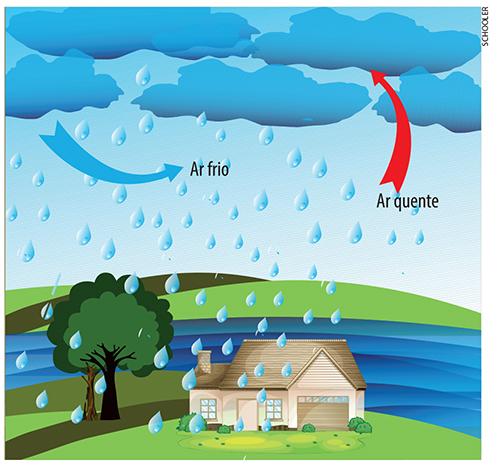
\includegraphics[width=0.55\textwidth]{Textuais/Figuras/chuva-frontal.png}
    \label{fig:frontal}
    \fonte{https://goo.gl/gfzp6t}
\end{figure}

As precipitações orográficas (também nomeadas de chuvas de relevo) ocorrem durante a ascensão de massa de ar quente e úmido, pelo encontro de um obstáculo (serras são um exemplo) forçando a elevar-se e, consequentemente, reduzindo a temperatura sucedendo a condensação, como mostra a Figura \ref{fig:orografica}. Este tipo de chuva ocorre em pequenas áreas, sendo de baixa intensidade e extensa duração \cite{ciclo-hidrologico}. Após a ocorrência da precipitação, algumas vezes, a massa de ar consegue transpor a barreira, projetando a sombra pluviométrica, caracterizada por regiões secas, devido à umidade já ter sido, em grande parte, descarregada no lado oposto \cite{chuva-orografica}.


\begin{figure}[h]
    \caption{Formação das chuvas orográficas}
    \centering
    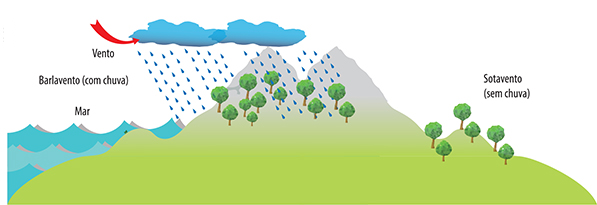
\includegraphics[width=0.85\textwidth]{Textuais/Figuras/orografica.png}
    \label{fig:orografica}
    \fonte{https://goo.gl/gfzp6t}
\end{figure}

Na classificação de precipitações convectivas, enquadram-se as chuvas intensas, típicas de regiões tropicais. A superfície aquecida, desigualmente, formam camadas de ar com densidades diferentes se mantendo em equilíbrio instável. Com a quebra desse equilíbrio (vento, superaquecimento), ocorre a ascensão brusca do ar menos denso, capaz de alcançar grandes altitudes, que atinge o nível de condensação e precipita \cite{hidro-aplicada}.